\section{A Model for Adversarial Testing}
The first challenge when performing safety validation is the setup of the problem. In this work we construct models as Markov Decision Processes as a convenient and consistent method of description. 

\todo{Move this to background and related work?}
A Markov decision process (MDP) is a model for sequential decision-making problems where an agent repeatedly takes actions in an environment which evolves stochastically over time. The state of the MDP contains all the information needed to fully describe the environment and the agent at a particular point in time. Consequently, MDPs have the \emph{Markov assumption} which means that the probability of transitioning to a state of the MDP depends only on the current state and the action of the agent. An MDP is defined by 5-tuple $(\mathcal{S}, \mathcal{A}, T, R, \gamma)$. The state space $\mathcal{S}$ represents all of the possible states that the agent and environment can be in and can be discrete or continuous. The action space $\mathcal{A}$ represents all of the possible actions that the agent can take and may also be discrete or continuous. The transition model $T(s, a, s^\prime) = P(s^\prime \mid s, a)$ gives the probability of transitioning to state $s^\prime \in \mathcal{S}$ given the current state $s \in \mathcal{S}$ and the action $a \in \mathcal{A}$. When implementing an MDP solver it can be useful to distinguish between \emph{explicit} MDPs, where the transition probability is explicitly defined via a function or a table of probabilities, and $\emph{generative}$ where the transition model is not explicitly known but can be sampled from. The reward function $R(s,a)$ provides feedback to the agent about the value of different actions and states. The discount factor $\gamma \in [0,1]$ is used to discount future rewards.

The goal of the agent is to maximize the expected discounted sum of future rewards, or \emph{utility}, from the current state $s$ given by
\begin{equation}
    U(s) = \mathbb{E}\left[ \sum_{t=0}^\infty \gamma^t R(s_t, a_t) \mid s_0 = s \right]
\end{equation}

\todo{Description of what a policy is}

The problem of safety validation assumes that we have an existing policy $\pi$ for an MDP and that at lease some of the stochasticity in the environment is controlled through a disturbance $x$ such that the transition function can be modeled as $P(s^\prime \mid s, \pi(s), x)$. Given these assumptions, it can be straightforward to formulate the safety validation problem as an MDP which we refer to as the \emph{adversarial MDP}. The adversarial MDP shares the same state space and transition model as the original MDP but the action space becomes the set of disturbances $\mathcal{X}$, and the reward function is designed to find failures. The choice of the discount factor will depend on the choice of reward function and the optimization algorithm used to solve the safety validation problem. Further discussion will be included for specific experiments and algorithms. 

the reward function will depend on the specific safety validation task at hand. To minimize confusion, let the reward function for the adversarial MDP be $R_{\rm adv}(s)$ and the reward function for the regular gridworld MDP be $R(s)$. If we care about falsification then the reward function of the adversarial MDP can be \num{1} if the agent arrives
\todo{Add the adaptive stress testing reward and the falsification reward}


The following sections describe several MDPs and the adversarial versions that will be used for experimentation in later chapters. These MDPs serve as good examples for demonstrating the process of describing an adversarial MDP as well as practical MDPs on which to test various safety validation algorithms. Each adversarial MDP has an associated Julia package for those interested in testing their own safety validation algorithms. 

\section{Gridworld Problems}
As is done in many treatments of algorithms for sequential decision making, we start with the gridworld. The gridworld is a simple MDP with a discrete state and action space that can capture the fundamental principles of sequential decision making. It therefore makes an excellent testbed for safety validation algorithms. 

\subsection{Simple Gridworld}
As pictured in \cref{fig:simple_gridworld}, the gridworld is defined on an $N_x \times N_y$ grid of states, each with a different reward.  The state of the system is the grid location of an agent and the action space of the agent is [\emph{up}, \emph{down}, \emph{left}, \emph{right}]. The agent can transition to any adjacent state that is not out of bounds of the gridworld. The transition function depends upon a parameter $p_{\rm success} \in [0,1]$ such that the agent goes in the direction of its action with probability $p_{\rm success}$ or a random direction is selected with probability $1-p_{\rm success}$. If the transition direction results in an invalid state then the agent remains in the same state. Once the agent arrives in a state with nonzero rewards, it will transition (regardless of its action) to a terminal state where it permanently remains receiving \num{0} reward, effectively terminating the MDP episode. 

\begin{figure}
    \centering
    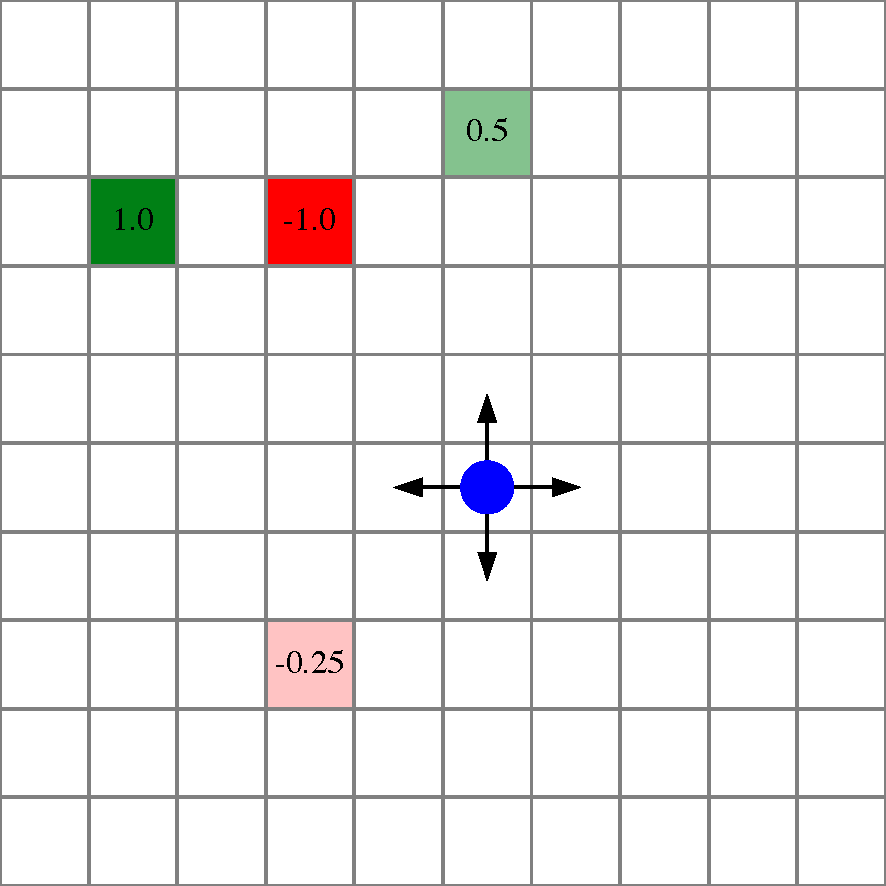
\includegraphics[width=0.5\textwidth]{figures/sample_systems/simple_gridworld.pdf}
    \caption{Gridworld MDP. Failure states are those with negative rewards.}
    \label{fig:simple_gridworld}
\end{figure}

An agent trained to perform optimally on this gridworld will learn a policy $\pi(s)$ that maps gridworld states to one of the four actions. 

To turn the gridworld into an adversarial MDP we must define what we mean by failure, determine what are the disturbances we wish to have control over and lastly, define a reward function. 

In the gridworld, a failure can be any time the agent arrives at a state with negative reward. 
An agent trained to behave optimally in the gridworld will only rarely reach such states so the probability of failure will be low
The disturbances are the stochastic transitions that the agent sometimes takes. If the adversarial MDP can control which transition happens to the agent, then we can discover sequences of transitions that end in failure. The probability of a disturbance is $p_{\rm success}$ if the disturbance is the same as the agent action, and $(1-p_{\rm success}) / (N_a - 1)$ otherwise, where $N_a = 4$ is the number of actions. 

The choice of reward function will depend on the specific safety validation task at hand (see section XXX for specifics). If we are interested in falsification or estimating the probability of failure, we may set the reward to be \num{1} for each failure state and \num{0} elsewhere. If we are interested in most-likely failure analysis then we can incoporate the probablity of each disturbance at each step. The specific reward function choices will be described for each experiment separately. 

This MDP and the adversarial version of it can be solved to an arbitrary degree of precision using dynamic programming, making it a good starting point for developing algorithms. 

The implementation of both the regular version and adversarial version of this MDP can be done using the \texttt{SimpleGridworld} MDP distributed as part of the \texttt{POMDPModelTools.jl}\footnote{TODO} package. The base MDP can be implemented by defining the grid size, the value and location of the rewards, the states to terminate from, and the probability of transition success. The adversarial MDP can then be constructed with the same size and terminal states, but the rewards are now set to \num{1} for each failure state in the base MDP and a probability of transition success as \num{1}. If the probability of the distrubance is important, then it can be computed from the policy under test and the probability of transition success of the base MDP.

\subsection{Gridworld with Adversary}

In order to increase the difficulty of the safety validation problem we introduce a new gridworld variation that includes an adversarial agent. The MDP is shown in \cref{fig:gridworld_with_adversary}. Two agents move on a gridworld: the ego agent (in blue) tries to reach states with high reward, while the adversary (in orange) tries to collide with ego agent. The dynamics of the gridworld are made more challenging for this problem by including impassible states (in black) and a larger action space [\emph{up}, \emph{down}, \emph{left}, \emph{right}, \emph{stay}, \emph{up right}, \emph{up left}, \emph{down right}, \emph{down left}].

\begin{figure}
    \centering
    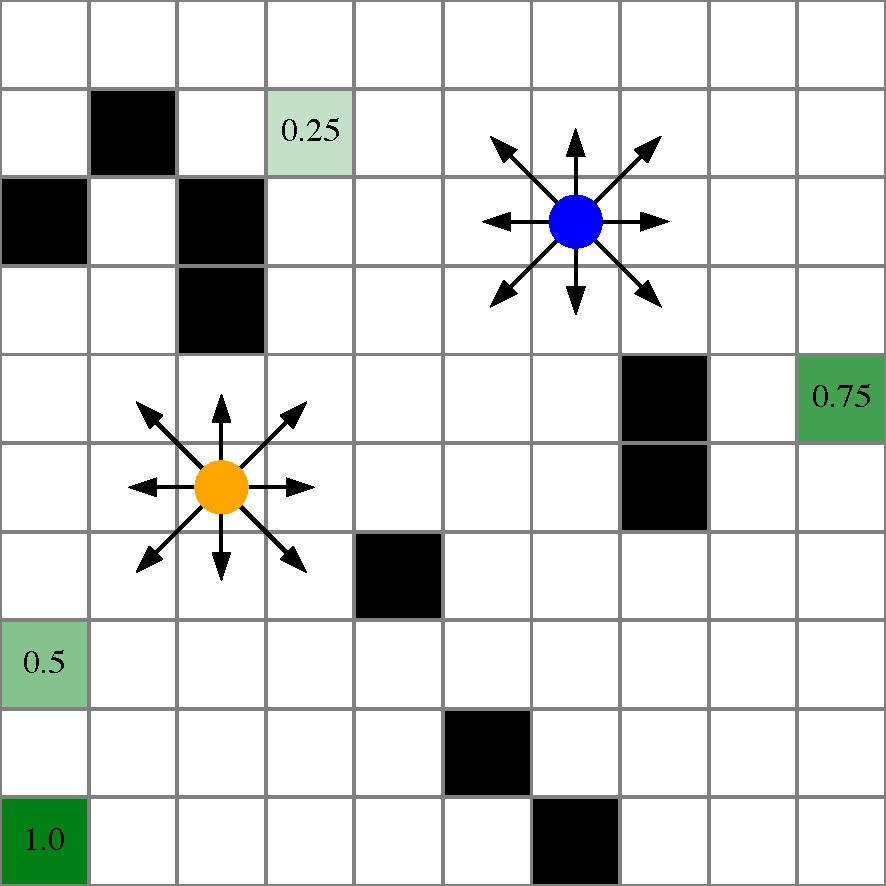
\includegraphics[width=0.5\textwidth]{figures/sample_systems/gridworld_with_adversary.pdf}
    \caption{Gridworld with Adversray MDP. Failure occurs when the ego agent and adversary collide}
    \label{fig:gridworld_with_adversary}
\end{figure}

The disturbances are the actions of the adversarial agent. the probability of each disturbance can be specified from a user-defined model of the adversary. For the experiments in this work, we assume that the true behavior of the adversary is uniform across the actions so each disturbance has equal weight. 

A failure of the ego agent is any time the adversary and agent overlap on the same state. 

The goal of this MDP is to increase the complexity of the safety validation problem while remaining tractable for dynamic programming solutions. 

Tunable adverarial policy

Both the base MDP and the adversarial MDP can be implemented using the julia package "AdversarialGridworld.jl"


\section{Autonomous Driving}
% Why autonomous vehicles
To complement the simplicity of the gridworld MDPs, we introduce two MDPs to model autonomous driving behavior in complex environments. Autonomous driving is an especially important domain for safety validation due to the recent development and deployment of autonomous vehicles~\cite{todo}. Safety validation of an autonomous driving policy is challenging due to the size of the state and disturbance spaces, the duration of the diving episodes, and the rarity of failure events.

% At a high level, how do we model
To model driving scenarios in simulation we build off of the julia package \texttt{AutomotiveSimulation.jl}\footnote{todo} which provides easy construction of road geometries, vehicles, pedestrians and behavior models. To facilitate the construction of adversarial MDPs for driving scenarios, we developed the package \texttt{AdversarialDriving.jl}\footnote{todo}. The adversarial driving MDP is construct from a set of agents where each agent is defined by
\begin{itemize}
    \item An \emph{initial condition function} that generates the initial state of the agent. The function may be deterministic or randomized, and is called each time the MDP is reset. 
    \item A \emph{behavior model} that determines the actions of the agent. For the system under test, this model implements the autonomous driving policy we wish to test. For adversaries, this model implements the disturbances that are being applied.
    \item A \emph{disturbance model} that is a probability distribution over disturbances which can be used to sample distrubances and compute their probability. 
\end{itemize}
The MDP is constructed with an agent representing the system, a vector of agents that act as the adversaries, a road geometry and the simulation timestep. The state and action spaces are dynamically constructed based on the number of agents in the scene and the reward function is specified based on the desired safety validation task. 




The driving policy that we employ is based on the intelligent driver model (IDM), a simple car-following algorithm that applies longitudinal acceleration to reach a desired velocity while avoiding rear-end collisions. 
\todo{Include the IDM code here}
The intelligent driver model assumes that the vehicle stays in the same during the simulation and does not include any lateral acceleration. With this assumption we can specify a vehicle's state using four state variables ($s$, $v$, $\ell$, $b$) where $s$ is the position along the lane, $v$ is the speed of the vehicle in the direction of the lane, $\ell$ is an integer representing which lane the vehicle is in, and $b$ is a Boolean that indicates if the vehicle's turn signal is on.

% What these MDPs do well
The upside to these MDPs is that they can model the continuous nature of states and actions in the driving environment, the complexities that arrive from multiple interacting driving agents, and rarity of failure events. The state and action space of each agent on the road is (at least in part) continuous, and multiple agents in a driving scenario leads to a exponential expansion in the number of states and actions. 

% What these MDPs don't do as well but why its still valuable.
They do not, however, model the potentially complex behavior of an industrial autonomous driving policy. Such agents are not currently widely available or tend to operate in simulators that are not appropriately outfitted for this style of safety validation. In order to make the results of these MDPs applicable to industrial autonomous driving policies, we attempt to match the size of the agent state and action spaces, the number of interacting agents and the rarity of failure events to an industrial simulator. It should also be noted that most industrial AVs use complex perception systems, which we abstract with simply models. Since the goal of this work is to stress test the planning modules of AVs then this abstraction seems acceptable.





\subsection{Pedestrian in Crosswalk}
In this MDP, we seek to the behavior of an autonomous vehicle approaching a crosswalk where a pedestrian is attempting to cross. The vehicle makes noisy observations of the pedestrian's position and velocity, and uses those observations as inputs to the IDM to determine the vehicle acceleration. The state space of the vehicle is ($s$,  

\begin{figure}
    \centering
    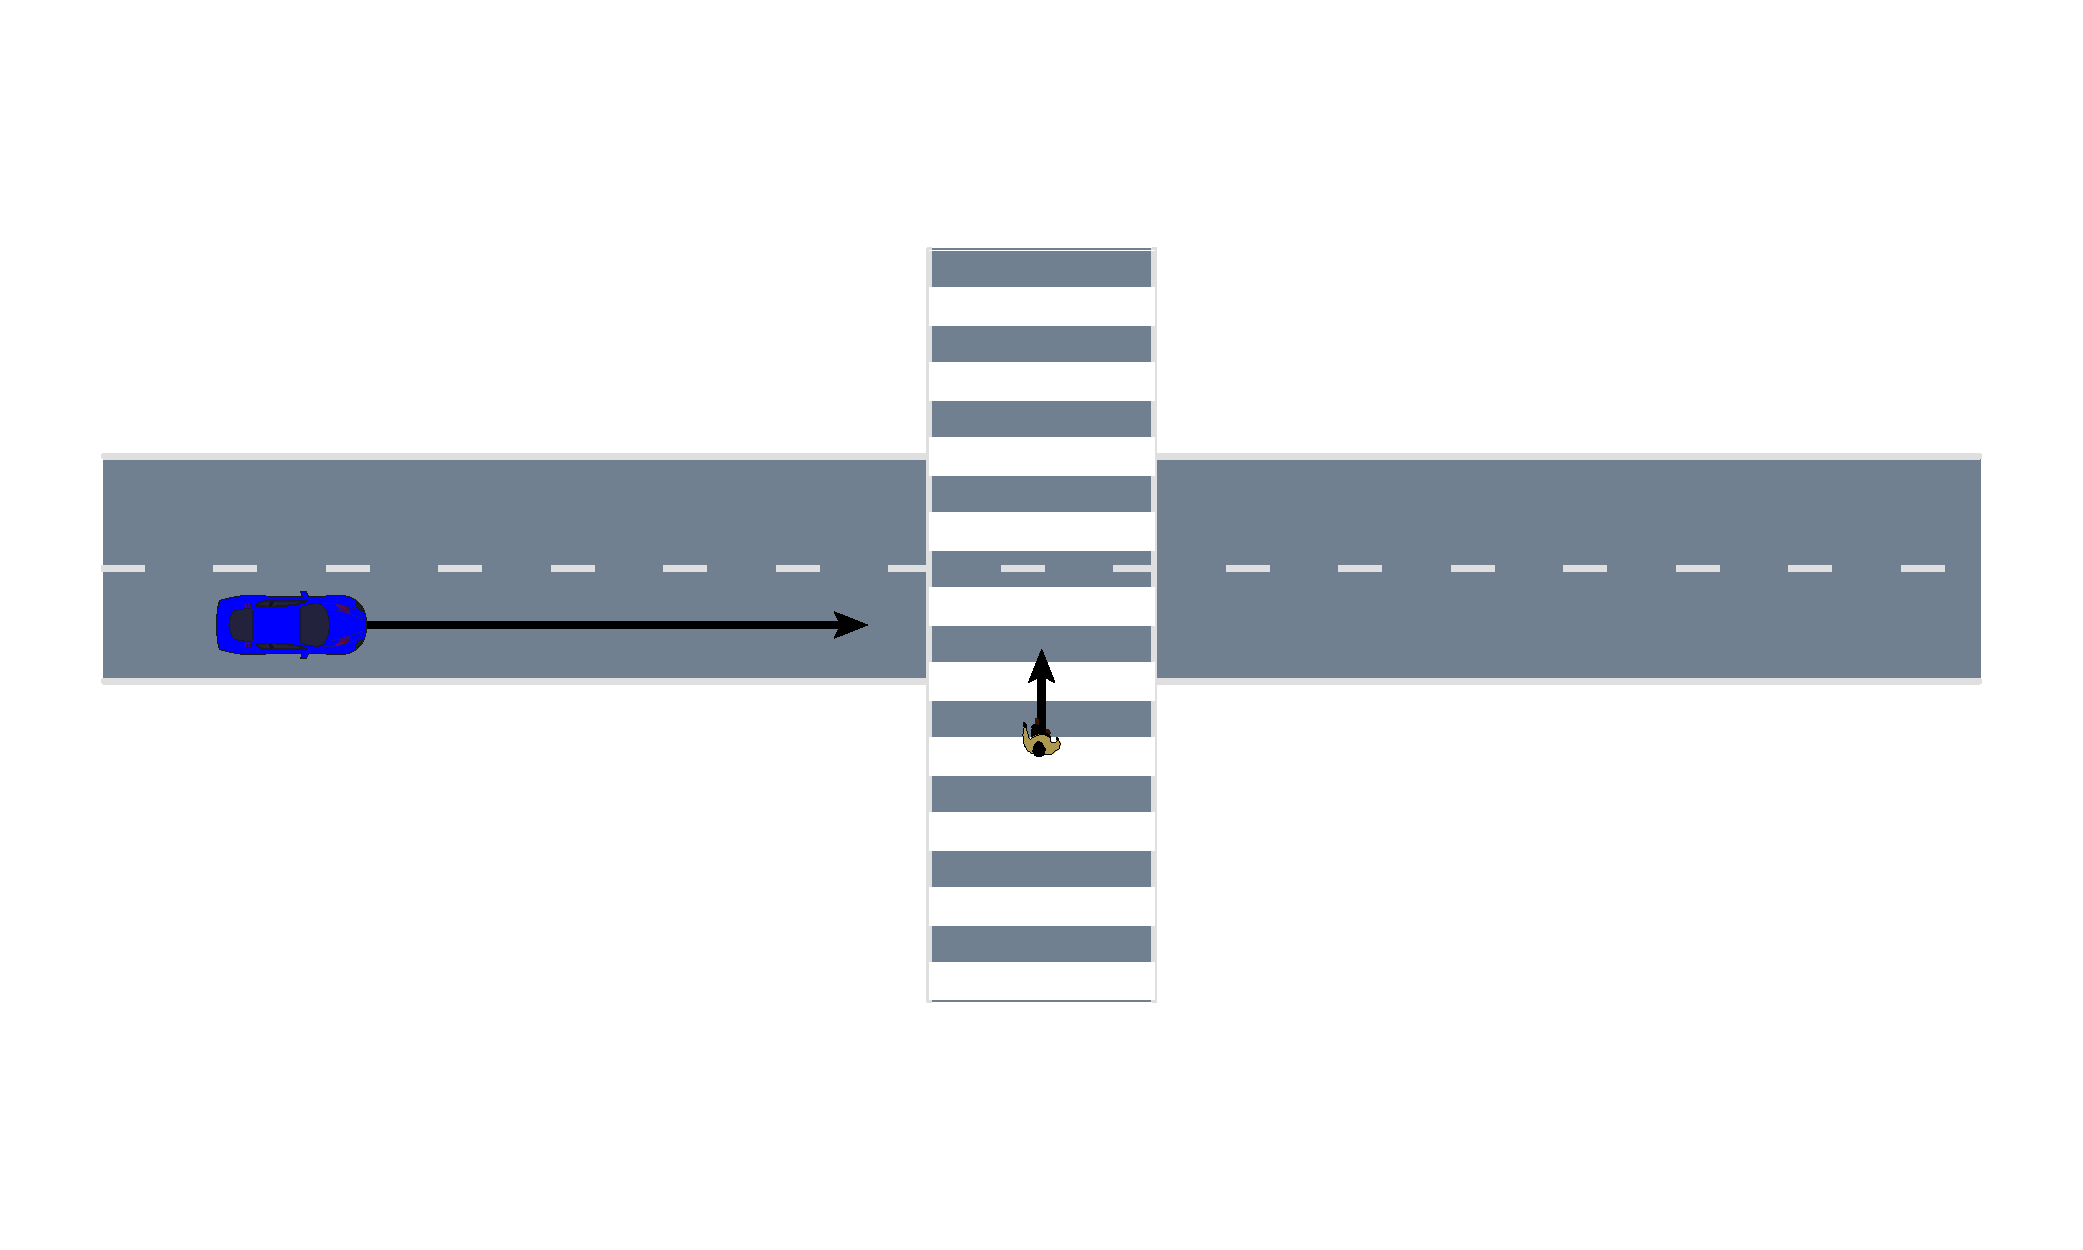
\includegraphics[width=0.7\textwidth]{figures/sample_systems/pedestrian_crosswalk.pdf}
    \caption{Crosswalk MDP. Ego vehicle approaches the crosswalk while a pedestrian tries to cross. }
    \label{fig:pedestrian_crosswalk}
\end{figure}

\subsection{T-Intersection}

\begin{table}
    \centering
    \caption{Action space for adversarial vehicles}
    \label{tab:adversarial_disturbance_space}
    \begin{tabular}{@{}lrr@{}} 
        \toprule
        \textbf{Action} & \textbf{Acceleration} & \textbf{MC Probability} \\
        \midrule
        No disturbance &  \SI{0}{m/s^2} & \num{0.976}\\
        Medium slowdown & \SI{-1.5}{m/s^2} & \num{1e-2}\\
        Major slowdown & \SI{-3}{m/s^2} & \num{1e-3}\\
        Medium speedup & \SI{1.5}{m/s^2} & \num{1e-2}\\
        Major speedup & \SI{3}{m/s^2} & \num{1e-3}\\
        Toggle blinker & N/A & \num{1e-3 }\\
        Toggle turn intent & N/A & \num{1e-3} \\
        \bottomrule
    \end{tabular}
    \vskip -0.2in
\end{table}


\begin{figure}
    \centering
    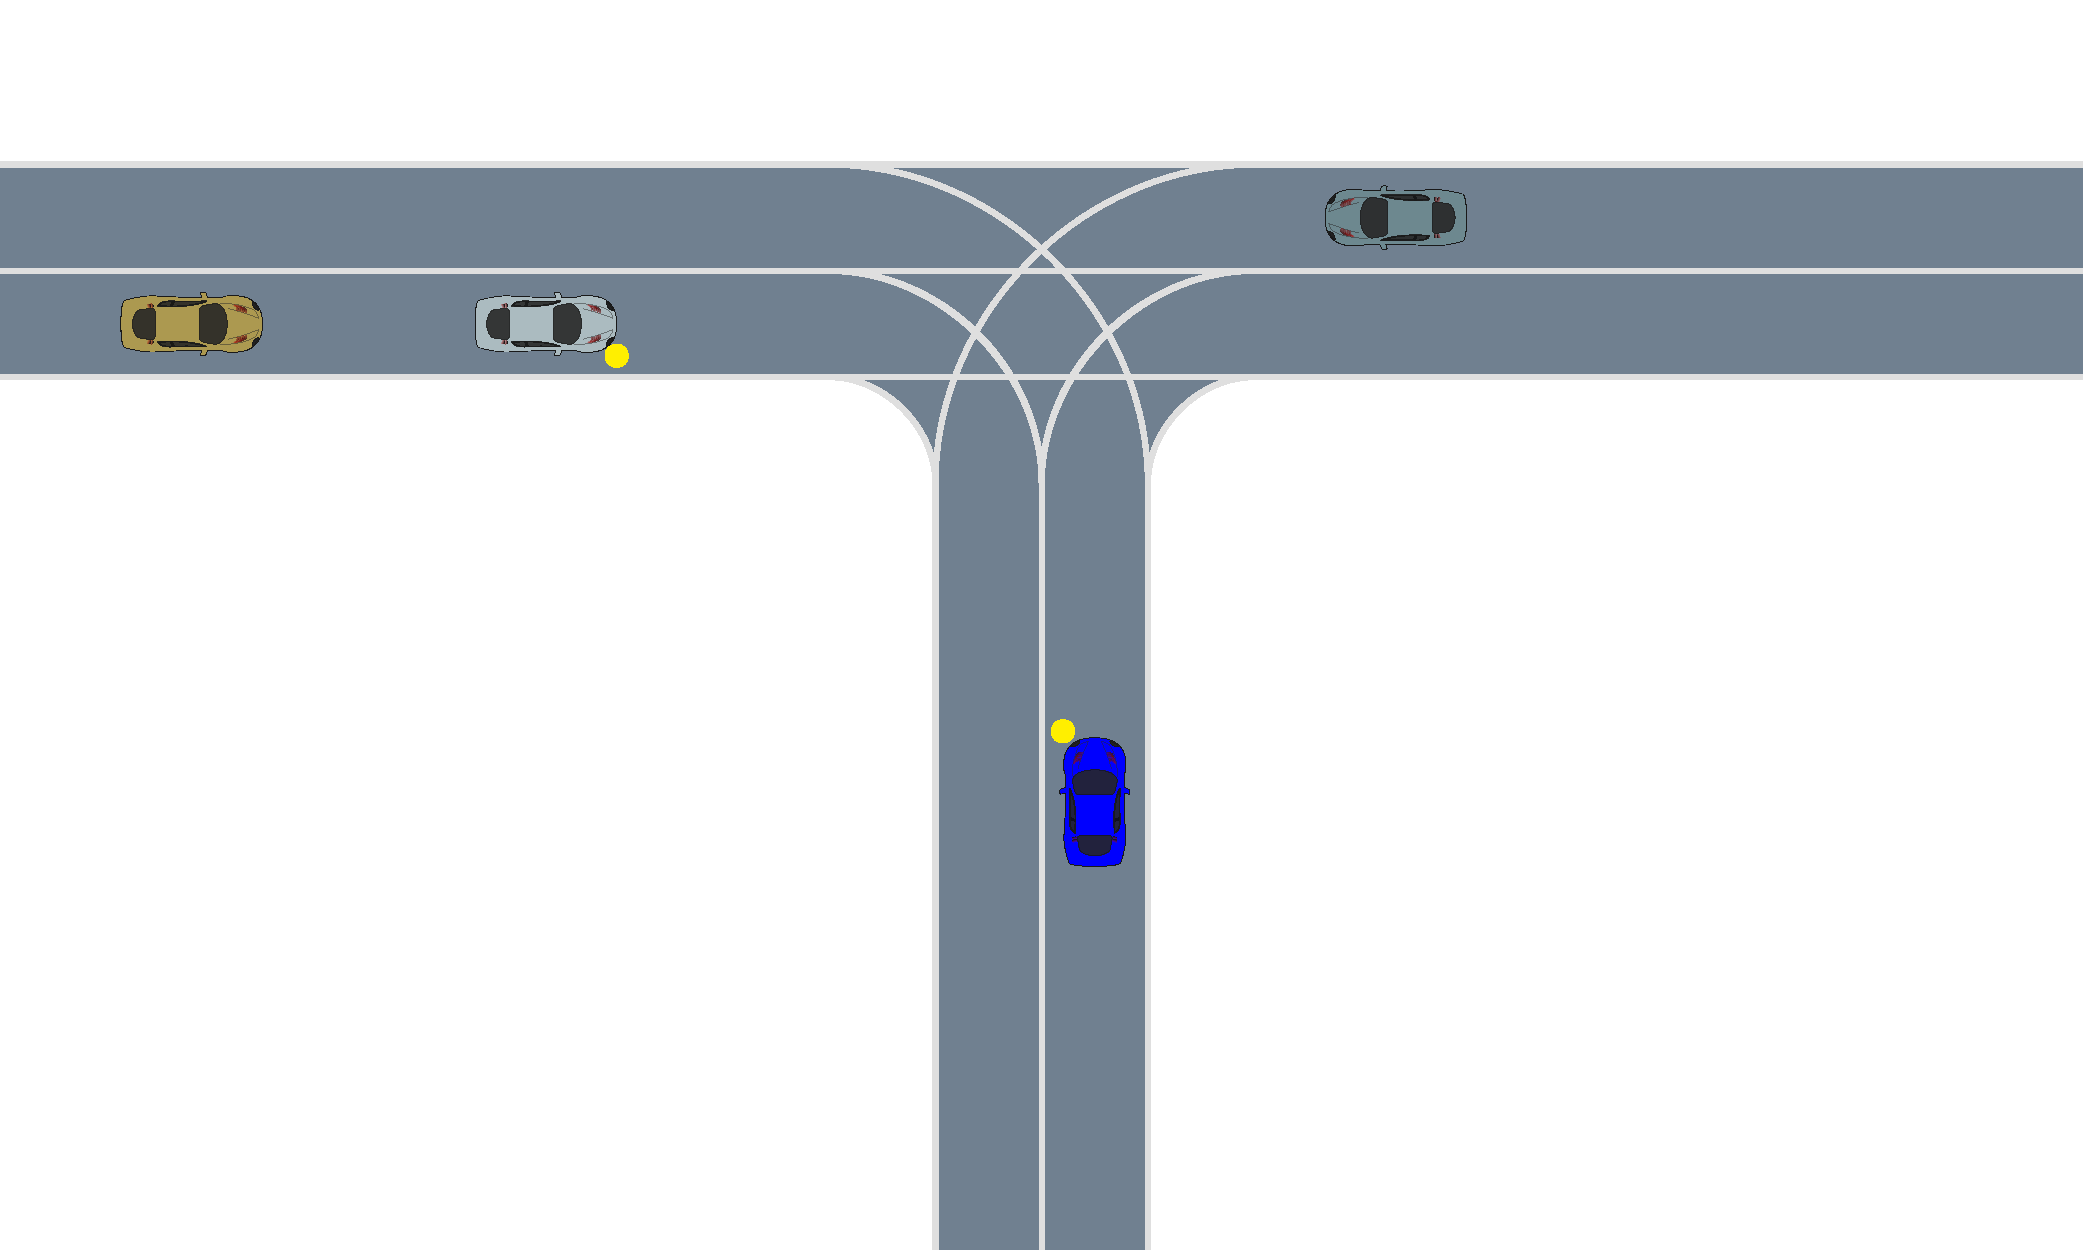
\includegraphics[width=0.7\textwidth]{figures/sample_systems/T_intersection.pdf}
    \caption{T-Intersection MDP. Ego vehicle tries to take unprotected left turn. }
    \label{fig:t_intersection}
\end{figure}

% Rules-based policy

 \begin{algorithm}
\caption{Intersection navigation algorithm}
    \label{alg:intersection_navigation}
\begin{algorithmic}[1]
    \footnotesize
    \Function{ComputeAcceleration}{$veh$, $scene$}
    \State $v \gets$ velocity($veh$)
    \State $v_{\rm lead}$, $\Delta s_{\rm lead} \gets$ leading\_vehicle($veh$, $scene$)
    \State $acc \gets$ IDM\_acceleration($\Delta s_{\rm lead}$, $v$, $v_{\rm lead}$) 
    \If{$veh$ does not have right of way} 
        \State $ttc$ $\gets$ time\_to\_cross\_intersection($veh$) 
        \State $\Delta s_{\rm int}$ $\gets$ distance\_to\_intersection($veh$)
        \If {$\Delta s_{\rm int} < \Delta s_{\rm lead}$} 
        \For{$agent$ in $scene$}
            \State $ttenter$ $\gets$ time\_to\_enter\_intersection($agent$) 
            \State $ttexit$ $\gets$ time\_to\_exit\_intersection($agent$) 
            \If{$ttenter < ttc$ and $ttexit + \epsilon > ttc$} 
                \State $acc \gets$ IDM\_acceleration($\Delta s_{\rm int}$, $v$, 0) 
                \State \textbf{break}
            \EndIf
        \EndFor
        \EndIf
    \EndIf
    \State \textbf{return} $acc$
    \EndFunction
\end{algorithmic}
\end{algorithm}

%Learned Policy
